%!TEX root =../../thesis-ex.tex

\chapter{Introduction}

With the rise of mobile devices, more than 70\% of the world population now own a mobile devices. Different from larger devices, users can easily carry these small devices on the go and perform different tasks such as searching for local restaurants, browsing news, replying emails, learning new languages, etc. Based on the statistics, mobile device subscription has surpassed that of laptop since 2016. As a result, more users access information on mobile devices rather than on desktops. Statistics show that in average, American adults spend approximately 4 hours a day interacting with their phones. Many of today's startup companies starts from mobile application and then move up to larger devices, because the mobile platform allows them to grow the business faster, i.e., mobile-first and mobile-only strategies. 

As a result, it is a critical task for business owners to make sure that user experience on mobile devices are friendly and user can effectively interact with information. In this thesis, we take the look at one problem in user interaction: users' decision making task on mobile devices. Due to the large number of mobile subscription, there has to be many cases where users need to make decisions and where their mobile devices are the only tool they can rely on. For example, consider a user traveling without the laptop and it happens to be Amazon Prime day where many products are on sale, or no Wi-Fi is available. With mobile devices, it is more convenient for them to catch the deals because if they need to wait until the desktop is available, they might have missed the deal. 

With the physical characteristics, however, it would be more difficult for the users to perform information seeking activities on mobile devices. Mobile screens are small and it is more difficult to type, edit or navigate on these devices. As a result, mobile devices are often where the users first research for a product. For example, after seeing an advertisement, they may become interested in buying a product and then start searching. Then they often end up buying it on their computers. Arguably, today it would still be more convenient to search and buy products on a computer. However, if we can improve users' buying experience on their phones, perhaps that makes them feel safer to make the decision over the phones, e.g., without having to miss the Prime day deal. 

How to improve users' decision making experience on their mobile devices? One key factor that determines decision making is how much information the user knows about the options. That said, decisions are frequently made out of uncertainty. Consider again the shopping example, which one is the optimal deal for the users' need? Theoretically speaking, the user can only know if for sure if she can traverse all the deals. However, on Prime day Amazon there might be millions of deals, so it is impossible to traverse them all. With keywords search, the user can browse through the top ranked items, but due to the screen size, difficulty for typing, etc., users would be more biased towards selecting the top ranked items, making it more likely for the user to make a suboptimal decision. 

Generally, the difficulty for users to reach the optimal shopping decision is caused by the knowledge gap between the user and the complete information that is required for decision making. The knowledge gap is a general problem that almost always exist with decision making. On mobile devices, this problem is further amplified by the difficulty for typing, editing, etc. Other decision making tasks on mobile devices include making business decisions (with business intelligence tools) and making security decisions by interacting with Android permission system. Similar as shopping, in both cases there exist knowledge gap which causes the difficulty in decision making. 

One approach for assisting users with decision making is to bridge the knowledge gap by supporting knowledge that the user potentially need to refer to for decision making. Compared with automated decision making, this approach would then be more friendly and explainable. The rapid growth of mobile industry has given rise to mobile data copora, e.g., 2.7 million apps are published on Android play store. Such datasets, as well as other mobile-related data (e.g., user mobile search data) provides an opportunity to support user decision making using data-driven approaches such as data mining, machine learning and information retrieval. In this thesis, we argue that \textbf{the massive and growing mobile-related meta datasets as well as user-generated data can be leveraged to computationally support user decision making by extracting such knowledge from these datasets}. 

This chapter is organized as follows. Section~\ref{ch1:sec1:background} introduces background and existing work on decision making support and mobile user interaction. Section~\ref{ch1:sec2:motiv} presents the motivation of this thesis. Finally, Section~\ref{ch1:sec3:overview} describes the organization of this thesis and summarizes each individual piece of work. 

%!TEX root =../../thesis-ex.tex

\section{User Decision Making on Mobile Devices}
\label{ch1:sec2:motiv}

With the prevalence of mobile devices, billions of users rely on mobile devices to fulfill their daily tasks. During interaction with mobile devices, users often need to face the challenge of \emph{making decisions}. That is, choosing between options, where the selection can affect users' personal benefit, e.g., money or security. Today, statistics suggest that more and more user decisions are made on smaller devices, e.g., statistics predict that by 2021, mCommerce will dominate the sales, with more than 53.9\% sales coming from mobile devices~\cite{mcommerce53}.

Decision making is a slow judgment process. Different from fast judgment tasks such as visual object recognition, speech recognition, slow judgment process often involves complicated mental models and user efforts in researching, exploration, learning new knowledge, and comparison. For example, when making shopping decisions for a product that they are unfamiliar with, users usually do not settle down on the first search result right away, but they need to researching information such as the price distribution for that product, what are the most popular name brands, etc, before finalizing the decision. For business decision, it may involve special programming skills such as querying a database. The lack of such knowledge thus creates a gap between user and the optimal decision. 

In general, the knowledge gap can be caused by the following reasons. First, \emph{transparency of the system}. When certain operations of the system cannot be known, from the users' side, it is difficult to make decisions based on the partially available or not available information, one example is security decision making on granting permissions where the user has no access to directly observing how exactly the permissions are being used, another example is AI systems that automatically make decisions for users. Second, \emph{decisions need to be made from a large database}. When decisions need to be made from a large database, it is impossible for the user to go through all the options, therefore even the system supports keywords search, it still possible that the user have missed some options, this problem is amplified if the keywords search function is poorly supported or it is difficult for the user to formulate a good query, one example is clothes search in a shopping website. Third, \emph{making decisions require specialized knowledge}. For example, when querying a database for making business decisions, a data analyst needs to know the grammar of SQL. Without other supports, it would be difficult for the data analyst to perform such queries. 

The knowledge gap for decision making on mobile devices is further amplified. As discussed in Section~\ref{ch1:sec1:background}, mobile user interactions are affected by its screen size, difficulty in typing and difficulty understanding permission requests. With \emph{typing difficulty}, it is more difficult for users to interact with search engines as like in computers. With \emph{smaller screens}, it is also more difficulty for users to navigate through the search results. Also with \emph{difficulty typing and editing}, users face more challenges searching for answers to difficult and technical questions, e.g., questions on coding tasks. Mobile systems also introduces its new decision scenarios, i.e., when requesting security permissions, users often do not understand the purpose behind such requests, for average users, without explanation by the app developers, it is very difficult for them to obtain such knowledge from other places, e.g., Google.

\section{Bridging Knowledge Gap for Decision Making}

One essential way for assisting users' decision making tasks is to suggest external knowledge to users before the decisions need to be made. Such knowledge support systems are often seen in information systems. For example, along with Google search results, the engine often actively suggest related knowledge entries, e.g., if the user searches for a shopping related query, the search engine not only display results that answers the query, but also related knowledge which goes beyond the query itself, e.g., how much a mattress box spring costs (Figure~\ref{ch1:fig2:knowledge1}). Such knowledge may help users make better decisions, e.g., by knowing how much a good box spring cost, users are less likely to pay more money than they need to. 

\begin{figure}[h]
\centering
\subfloat[][``People also ask'' (both desktop and mobile)]{\includegraphics[width=.6\textwidth]{figure/chapter1/knowledge1}\label{ch1:fig2:knowledge1}}\hfill
\subfloat[][``Interesting finds'' (mobile only)]{\includegraphics[width=.3\textwidth]{figure/chapter1/knowledge3}\label{ch1:fig2:knowledge2}}
\caption{Google actively suggest knowledge entries to help users making decisions}
\end{figure}

On mobile devices, by realizing the knowledge gap, Google has further enhanced the knowledge support. Besides also displaying the knowledge entries as on desktop, Google further enriches the mobile search results, including showing ``interesting finds'' (Figure~\ref{ch1:fig2:knowledge2}). In general, Google's mobile search results is much more diversified than desktop search results. 

Knowledge support is also often seen in clinical decision support systems, where the system helps users to retrieve medical documents, disambiguate difficult medical terms and answer questions~\cite{sankhavara2018biomedical}. 

The general methodology behind knowledge assistance include the follows. First, \emph{retrieval}. If the knowledge entry is a natural language sentence, it can be directly retrieved from a candidate corpus by defining a scoring function. When the suggested knowledge can be directly adopted from the original data, and when the data size is large enough, retrieval has many advantages, including efficiency, good interpretability and low cost. Notably, with retrieval approaches, labeled data can be leveraged but it is not required. For example, retrieval-based question answering is often used in question answering systems. Second, \emph{summarization}. Sometimes the user needs to get a knowledge of the data distribution of the corpus, where summarization could help. For example, histogram summarizes the distributional statistics of the corpus. Topic models summarizes the main content in the documents. Third, \emph{generation}. Different from retrieval, generation can be applied even when the dataset does not contain the answer to the question being answered. 


%!TEX root =../../thesis-ex.tex



\section{Background}
\label{ch1:sec1:background}

\subsection{Studies in Decision Making}



\subsection{Traditional Decision Support Systems}

\subsection{Data-Driven Information Systems}

Search engine and recommender system are the two major types of information systems that users frequently interact with for making decisions. Such work mostly inspires the methodology of this thesis on how to develop data-driven models to support users for making decisions. 

\textbf{Learning from User Click Logs}. User click through logs are regarded as partial relevance feedback, therefore they can be used to train machine learning and neural network models which effectively improve the performance of actual ranking results compared with non-learning approaches. Such models are further improved, because the clicks themselves may not directly reflect user satisfaction. For example, if the user visits a link for less than a few seconds, it is less likely that she has found the relevant information from that link. As a result, people have proposed to focus on clicks with longer dwell time (e.g., exceeding 30 seconds) which are more likely satisfied clicks~\cite{kim2014modeling}. On the other hand, even if the user skips a result, it does not necessarily mean it is non-relevant. It may be because the relevant information need already appeared on top. To further improve the model, \cite{Craswell:2008:ECC:1341531.1341545} proposed a cascade model which captures the probability for skipping the top results. 

\textbf{Leveraging Other Data Resources}. In information systems, meta data/additional user generated data can often help with search/recommender system optimization, especially when no query is available or the query is too simple. For example, user's biographic features, such as name, gender, can help with improving the performance of personalized recommender system. User review data, provides crowd sourced opinions that helps with identifying high quality results. For instance, leverage topic modeling on products review data to improve the matching probability between query and products, as products are structured data which often lacks opinionated descriptions as in the queries, e.g., \emph{quiet fan}~\cite{duan2013probabilistic}. User review data can also support aspect based search to cater users' fine grained needs, e.g., when searching for hotels, some users consider location an important factor, while others care more about price. 

% \textbf{Formal Models of Users' Information Seeking Behaviors}. Researchers have built different models to capture users' information seeking behavior. An early model proposed by Pirolli and Card compares users' information seeking process with predators (user) hunting for food, where predators consume energies (searching and browsing) in hoping to finally reach the food (information need is satisfied). In web search and browsing, users behaviors consists of frequent switches between searching, scanning highlights, visiting websites, consumption of the contents, leaving sites, etc., until the user's information goal is reached or the user gives up. During these processes, it is the \emph{information scent} that supports users to go deeper, for example, relevant texts and highlighted words on search engine result page give users the promise that they may eventually get the ``food'' by visiting a website. In other words, unless user finds the scent stronger and stronger along the path (i.e., improved quality), she will give up the process. Such theory had turned into concrete guidelines to help websites improve the designs. It also inspired Google to re-rank the search results~\cite{Nielson2003Forage}. Following the information scent work, researchers at PARC develop an automated usability testing tool called Bloodhound~\cite{chi2003bloodhound}, which uses a probabilistic model to measure the easiness for user to reaching the desired destination. User studies show that the proposed measure agrees with users' real responses.

% Information foraging theory was adopted by more recent work in formal models of users' information seeking. SNIF-ACT~\cite{fu2007snif} test user actions in a world wide web setting. \cite{chi2010method} further developed methods for highlighting texts. Multiple systems was proposed to estimate the semantic relatedness to simulate information scent~\cite{budiu2007modeling}, e.g., latent semantic analysis by (LSA~\cite{landauer1997solution}). Information scent was also applied to the scenario of software development~\cite{lawrance2008using}. The theory inspired a list of work on using simulation to replace human usability testing to reduce the cost of testing~\cite{chi2003bloodhound,carterette2015dynamic}. For example, \cite{carterette2015dynamic} simulates a complete set of behaviors, including clicks, dwell time, abandonment, and query through probabilistic models. \cite{luo2014win} presents a similar idea by modeling the transition of search engine states using partially observable Markov decision processes (POMDP). 

% More recently, researchers have developed other formal models for the users' interactive searching process~\cite{conf/sigir/ZhangZ15,zhang2016sequential}. In these models, the search process is modeled as a collaborative game playing process between user and the search engine. The two parties take turns to play a card, and the goal is for them to achieve the best reward with the least cost. Such models are general enough to not only model the web search process of ten blue links in the search engine result page, but they can also be extended to the case of mobile search when SERP is not available, and when the interface consists of more components to support navigation~\cite{zhang2017information}. When playing the card, the search engine can update the interface in real time by actively choosing between showing the content and showing the navigation component, which is beneficial when querying plays a less important role, e.g., news browsing.  

\subsection{Mobile User Interactions}

The last decade witnessed a revolutionary increase in mobile market, the penetration rate almost doubled within the 10 years between 2007-2017, making more than 66.53\% of the world population own a mobile device in 2019~\cite{phone_penetration}. Statistics show that people spend approximately 4 hours a day on their phone. Because we have developed such a close relationship with our phone, researchers have been working on studying how users interact with mobile phones and how we can optimize such interactions. For example, a significant proportion of the SIGCHI proceedings each year are related to user interactions with mobile devices (Figure~\ref{ch1:fig1:sigchi_stats}). 

\begin{figure}[h]
\centering
\subfloat{
\begin{tikzpicture} [scale=0.9]
\begin{groupplot}[group style={group size= 1 by 2},height=5cm,width=10cm]%[ybar stacked,xtick=\empty,]%ytick=\empty]
\nextgroupplot[ybar,symbolic x coords={2006, 2007, 2008, 2009, 2010, 2011, 2012, 2013, 2014, 2015, 2016, 2017, 2018, 2019},legend style={at={(0.5,-0.2)},anchor=north, ymin=0, ymax=120,legend columns=2},  ymajorgrids = true,bar width = 4.5,xtick=data, x tick label style={rotate=45,anchor=east}]%ytick=\empty]
\addplot[fill=black,draw=black] 
coordinates {(2006, 24.0) (2007, 23.0) (2008, 24.0) (2009, 31.0) (2010, 37.0) (2011, 50.0) (2012, 52.0) (2013, 49.0) (2014, 78.0) (2015, 75.0) (2016, 68.0) (2017, 73.0) (2018, 100.0) (2019, 81.0)};
\end{groupplot}
\end{tikzpicture}
}

\caption{Number of SIGCHI proceedings over the years with title containing the word \emph{mobile} or \emph{phone}\label{ch1:fig1:sigchi_stats}}
\vspace{-0.2in}
\end{figure}

Mobile devices differ from laptop/desktop computers in many aspects, including both the operating system and the user interface. For both aspects, researchers have studied the impact of such difference on users' interactive behaviors. 

\textbf{Users' Mobile Search Behaviors}. Compared with desktops/laptops, mobile devices have much smaller screens and it is easier to make mistakes during typing. As a result, users often show very different search behaviors. 

Previous work conduct large-scale empirical studies on Google~\cite{kamvar2006large} and Yahoo! search logs~\cite{yi2008deciphering}. The former study found that users' exploratory behaviors in mobile searches are largely lowered~\cite{kamvar2006large}. Previous work has not found a large difference in query lengths on mobile devices and computers, but compared with on mobile devices, users tend to reformulate more queries in the same session on computers~\cite{kamvar2006large}. Such results are consistent with the fact that mobile typing is more difficult than typing on computers. Another work used eye-tracker to record the difference between the eye movement behaviors on mobile devices and computers~\cite{kim2015eye}. They find that users exhibit slower eye movements on mobile devices than on computers. However, they experience more difficulty extracting information on mobile devices, and users are more likely to focus on top-ranked results on mobile devices. Users' mobile search behaviors also verifies the theory of information scent, where researchers found that mobile searchers need an increased amount of relevant search results, while desktop searchers are more accurate when each page contains an equal number of relevant search results~\cite{ong2017using}. Another behavior difference lies in \emph{good abandonment}, which means the user already finds an answer in the search engine result page, therefore the information need has been satisfied before any clicks. Researchers found such behaviors more frequent on mobile devices~\cite{williams2016detecting}. As a result, user satisfaction is not determined solely by clicks, therefore they propose to use gesture features to estimate users' satisfaction.  

The difference between mobile and desktop/laptop computers has also inspired research of actionable results. \emph{Summarization}. With smaller screens, mobile information systems no longer display the complete long text description as on desktop, e.g., the title of e-Commerce products can be summarized to better fit in the smaller screen on mobile devices~\cite{sun2018multi}. \emph{Search result diversification}. Since mobile users lack exploration and query reformulation, the search engines provide remedies. Notably, the search results on mobile devices are more diversified than on computers to encourage exploration. \emph{Enhanced query auto completion}. As researchers observe the difficulty for typing, they propose a term-by-term strategy for auto completing queries, different from the standard strategy which suggest the whole query at the same time~\cite{vargas2016term}. \emph{Context-aware Results}. The location of user provides information that could be leverage to improve the results in multiple aspects~\cite{lin2017location}. \emph{Slow search}. As mobile search tends to be slower than desktop search due to the network condition or other factors, researchers proposed to include higher quality results trading off the delay time.

\textbf{User Behaviors towards Mobile Applications}. Besides the search engine, a major part of mobile user interaction is with mobile applications. Mobile operating systems are dominated by iOS and Android, where Android has more than 76\% of the market share. As of 2019, Android has released its 10th version (Android Q). 

A large part of the user behavior studies on mobile applications focus on their behaviors towards security and privacy operations. Because such operations directly affects users' own security, users often need to spend time making decisions, therefore users' security response can lead to direct implication which helps system and application developers improve the security of the system. 

In 2011, researchers found that users were confused by Android permission requests, having trouble making decisions on whether to grant permissions for an application~\cite{conf/soups/FeltHEHCW12}. This behavior is due to the design of Android system, where applications must ask for permissions from the user before they can get access to the corresponding resources. The user, as a result, must decide whether to grant permissions to an app. If a permission is unrelated to or looks like it is unrelated to an app's main functionality, it is hard for the non-expert user to determine whether it is a case of \emph{over-privilege} or not (i.e., the application requests more permissions than it needs to). In particular, \cite{conf/soups/FeltHEHCW12} found that more than 1/3 of the apps contain at least 1 application that could not be understood by the user. 

Over the years, Google has released multiple new versions of Android permission systems. After Android 6.0 (Marshmallow), the permission model was replaced by a new model where each permission is requested one at a time and during runtime. This design makes it easier for application developers to embed the permission request in context, e.g., requesting location with the background showing a maps makes it easy to understand the motivation. The new system also allows users to turn off a permission after previously granting it. However, researchers still found users' difficulty in understanding permissions~\cite{}, especially with background usages~\cite{background}. 


%!TEX root =../../thesis-ex.tex

\section{Definition of Decision Making and Decision Support Systems}

In this thesis, we consider both user decision and decision making as their most general sense possible. Decision making is the activity for a user to interact with systems on her device, where the user have to choose from a set of options, and the selection is related to the users' personal benefit, e.g., money, security, or a significant amount of time. 

Under this definition, most activities for the user to interact with an information system (i.e., search engine or recommender system) are within the scope of decision making. For example, when a user needs to make selection for which paper to read next, or which movie to watch next, it may require a significant amount of time, therefore these activities should also be categorized as decisions. Interactive activities that we do not consider as decisions are tasks where the interactions are fixed and without much uncertainty, e.g., the how-to activities such as how to attach a photo to a Tweet. 

Similarly, we consider decision support systems a general concept. A decision support system is any system that provides information more than the original information and assist users reduce the uncertainty of decision making. As a result, any recommender system (e.g., people who bought this also bought) is a decision support system under our definition, because the suggested items allows users to observe similar items more efficiently which could potentially lead to a purchase decision. A question answering shopping agent is also a decision support system because it helps the users to reduce the uncertainty for a produce. Therefore, the decision support can be in two ways: first, the system initiate the decision support by actively providing information; second, the system support decisions on demand and provide the information specified by the user. 

\section{Motivation for Three Decision Making Problems Studied}
\label{ch1:sec3:overview}

Despite the work done by Google on knowledge support on mobile devices, there still exists many problems where such knowledge is not available on mobile results for bridging the gap, or the provided knowledge entry can be further optimized. In this thesis, we study knowledge support for the following three decision making challenges for mobile users. 

\textbf{Assisting Shopping Decision Making}. Users' shopping decisions often involve the need for them to understand and manage complicated product features, e.g., to purchase a computer, the user needs to know what brands she wants to purchase, her budget and what is the price distribution of the products, or even the relation between price and features, e.g., \emph{what is the minimum price I need to pay for a computer with 16GB ram?} Without knowing such knowledge, it is more challenging to issue a meaningful query. For example, the user may want to add to the query a brand name which she saw 10 products above the current position. With mobile screens, it can be more difficult to navigate that product. On the other hand, when completing the query, the query expansion results overrides the search results, making it more difficult to edit the query while viewing the products at the same time. 

\begin{figure}[h]
\centering
\subfloat[][Desktop showing search results and query suggestion at the same time]{\includegraphics[width=.65\textwidth]{figure/chapter1/overview2}\label{ch1:fig2:overview2}}\hfill
\subfloat[][Mobile showing query suggestion only]{\includegraphics[width=.27\textwidth]{figure/chapter1/overview1}\label{ch1:fig2:overview1}}
\caption{The difference in query expansion interfaces on desktop and mobile: desktop displays the search results and query expansion at the same time; on the other hand, mobile query expansion page overrides the search results, therefore it is more difficult to add keywords to the query, e.g., \emph{zinus}}
\end{figure}

To support user navigation on mobile devices, e-Commerce apps often provides a faceted search system, which shows ranked lists of the meta data of products, e.g., brands, price distribution, screen sizes. By navigating the system, the user does not need to remember the features, but can directly click on the facet values to filter the results, e.g., \emph{brand = Dell}. 

Faceted search system makes navigation on mobile devices easier, however, by the time the study was conducted, an important component had not been optimized, which is the numerical facets of products. As discussed above, users often need to learn the price distribution of a product before making a salient decision. The numerical facets also helps users more conveniently navigate to the subset of products whose prices are within the ranges more relevant to users. By the time the study was conducted, however, a majority of numerical facets are predefined, so that the website shows the same price distribution for diamond ring and greeting cards. The same results offer no clue for price distribution of these products. Meanwhile, it also increases the difficulty for navigation. As a result, for the first problem, we study the problem of optimizing numerical facets for assisting shopping decision making. 

\textbf{Assisting Security Decision Making}. Mobile systems introduce a new decision making task for users: security decision making. Android permissions control the access for mobile applications to access users' private data resources, e.g., user location, contact list. In the earlier versions of Android, the permissions are requested during installation time (Figure~\ref{ch1:fig2:android1}), and users must accept those permissions before they can install the app. Meanwhile, the system does not support any explanation to be added to the interface in Figure~\ref{ch1:fig2:android1}, therefore the knowledge support for decision making was not possible by design. In Android 6.0 and later (Android Marshmallow), the permission system was replaced by a runtime model, where the permission requests can be postponed until it is used during runtime (Figure~\ref{ch1:fig2:android2}). This new design thus allows the knowledge support to appear by inserting a new layout before or after the permission request. The latest version of Android (Android Q) keeps the runtime permission but also allows the install time permission to be granted individually, so that users have more opportunities to make decisions. iOS has a similar permission requesting interface, but more conveniently, the developer can display the explanatory sentences right on the permission requesting page. 

\begin{figure}[h]
\centering
\subfloat[][Install-time Permission]{\includegraphics[width=.25\textwidth]{figure/chapter1/android1}\label{ch1:fig2:android1}} \hskip 40pt
\subfloat[][Android M (Runtime)]{\includegraphics[width=.25\textwidth]{figure/chapter1/android2}\label{ch1:fig2:android2}} \hskip 40pt
\subfloat[][Android Q]{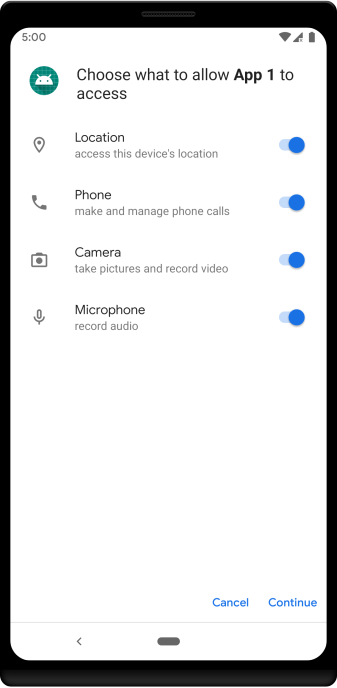
\includegraphics[width=.25\textwidth]{figure/chapter1/android3}\label{ch1:fig2:android3}}
\caption{The three Android permission models: install-time permission (all permissions are requested at install time); runtime-permission (permission can be delayed at the runtime); and the latest permission model (permissions can be requested at both the install time and runtime permission)}
\end{figure}

Although the newer permission models have allowed the applications to support knowledge to users for making security decisions, such changes do not guarantee that developers \emph{will} provide such knowledge. Indeed, we can always find news articles or forum posts complaining that Android permission purposes are confusing. As a result, we propose to study two problems: first, have Android apps provided sufficient knowledge supports for users' security decision making; second, if not enough knowledge are provided, how can we assist developers to improve the decision support. 

\textbf{Assisting Data Analytics for Business Decision Making}. A general strategy to support users' decision making, especially business decisions, is to support data analytics, including database queries. For example, the user may want to make a decision according to last years' sales record. On desktop/laptops, the decision making usually involves querying of a database. However, novel data analytics may not be familiar with SQL grammar. As a result, it would be convenient to support a natural language interface to assist the decision making. Figure~\ref{ch1:fig5:powerbi1} shows an example of such a natural language interface. When the user input the natural language question ``what is the breed of the dog named betty'', the system translates it into an SQL statement: \texttt{SELECT breed FROM dogs WHERE name = betty}, and displays the execution result. 

\begin{figure}[h]
\centering
\subfloat[][Conversational data analytics tool in Power BI (desktop)]{\includegraphics[width=.5\textwidth]{figure/chapter1/powerbi1_crop}\label{ch1:fig5:powerbi1}} \hskip 40pt
\subfloat[][Power BI iOS]{\includegraphics[width=.25\textwidth]{figure/chapter1/powerbi2}\label{ch1:fig5:powerbi2}} 
\caption{Microsoft Power BI interface (left) and the corresponding mobile application (right)}
\end{figure}

Mobile business intelligence is a new area (less than 10 years). However, surveys show that in 2017, 28\% percent of BI users stated that mobile BI was already in use in their company, with 23\% planned to be in use in the next 12 months and 22\% planned in the long term~\cite{mobilebi}. As of 2019, many mobile BI tools are in use. For example, Microsoft Power BI introduced the iOS application in 2015. Similar as the desktop version, the mobile applicaion also support the natural language interface feature (Figure~\ref{ch1:fig5:powerbi2}). 

To assist mobile users with business decision making, it thus is an important task to support natural language interface, i.e., translating the users' natural language question into SQL statement. Due to the aforementioned difficulty in mobile user interaction (i.e., small screen, difficulty researching information), it may be particularly difficult to write a correct SQL statement, therefore the support of natural language interface is particularly helpful. 

In these BI platforms, the NL2SQL must adapt to new database schemas provided by the user. As a result, the predictor must be able to generalize to new domains which has not been seen in the training data. The problem of cross-domain NL2SQL with complex query structure is still an active research area that has not been well solved. The problem of State-of-the-art approaches can achieve an accuracy of 65.5\%. As a result, we study the problem of translating natural language to SQL for cross-domain complex queries. 

\section{Organization of This Thesis}

The rest of this thesis is organized as follows. 

$\bullet$ \textbf{Chapter~\ref{ch2:shopping}: Assisting Shopping Decision Making with Numerical Faceted Search}. We study the problem of optimizing numerical facets to support users' shopping decision making on mobile devices. With a 2-month user query and click log on \url{www.walmart.com}, we develop a machine learning algorithm that suggests numerical ranges given a query. First, we propose an evaluation metric that evaluates the performance of a numerical range suggestion algorithm (Section~\ref{ch2:metric}). Based on the proposed metric, we propose three optimization algorithms by optimizing the metric directly (Section~\ref{ch2:dp}) and its upper bound (Section~\ref{ch2:percentage}). 

$\bullet$ \textbf{Chapter~\ref{ch3:runtime}: Empirical Study on Knowledge Support for Security Decision Making}. Before studying assisting users' mobile security decision making, we need to first empirically study whether existing applications have already provided sufficient explanations to support such decision making. Using sentence classification techniques, we creates a new dataset containing the explanation sentences by mobile applications. We propose five research questions to evaluate the sufficiency of explanations. Statistical significance tests show that generally, the decision support has not been sufficient compared with the suggestions by Android developers documentation. 

$\bullet$ \textbf{Chapter~\ref{ch4:clap}: Recommending Explanation to Assist Security Decision Making}. By identifying the deficiency in decision support, we propose to assist application developers to improve their existing explanations. By leveraging a large dataset containing the meta data of 1.45 million Playstore applications, we collect a large scale text corpus. By leveraging information retrieval techniques and unsupervised truth finding, our recommender system can suggest highly relevant sentences to the true purpose of the application. Qualitative evaluation shows the suggested sentences show three characteristics of interpretability. 

$\bullet$ \textbf{Chapter~\ref{ch5:nl2sql}: Assisting Business Decision Making with Natural Language to SQL Interface}. We study the problem of how to help mobile BI by supporting the natural language interface (NLI, or NL2SQL). We leverage a large complex cross-domain dataset named Spider to more closely simulate the scenario of mobile BI. By leveraging database values, we successfully matched database values that has been mentioned in the natural language question. We inject the matched database values to the existing state-of-the-art model on Spider, and observe 2.7\% improvement in the exact matching accuracy of output SQL statement. We further conduct an empirical study~\ref{ch5:sec:study} to explore potential ways for further improvement. 
